\section{\secState{D}Specialization of Hybrid Automaton}\label{s:MovementAutomatonBuidlingBlocks}

\paragraph{Idea:} There is  a need for \emph{fast trajectory approximation} method. The basic idea is taken from the pilot steering a plane. The pilot has issued commands from a navigator in a very short and precise manner. The movement has its primitive phase when steering is static, and its transition phase when steering is moving from one static position to another. 

Imagine having vertical and horizontal flaps an on airplane (fig. \ref{fig:movementsExample}). The \emph{navigator} is issuing a command every second to a pilot. Hands of the pilot translate each command to an input signal (blue line). The command validity period (black frame) is split into \emph{transition period} (red frame) when the input signal is changing and primitive period (magenta frame) when the position of the input signal is static.
 
\begin{figure}[H]
    \centering
    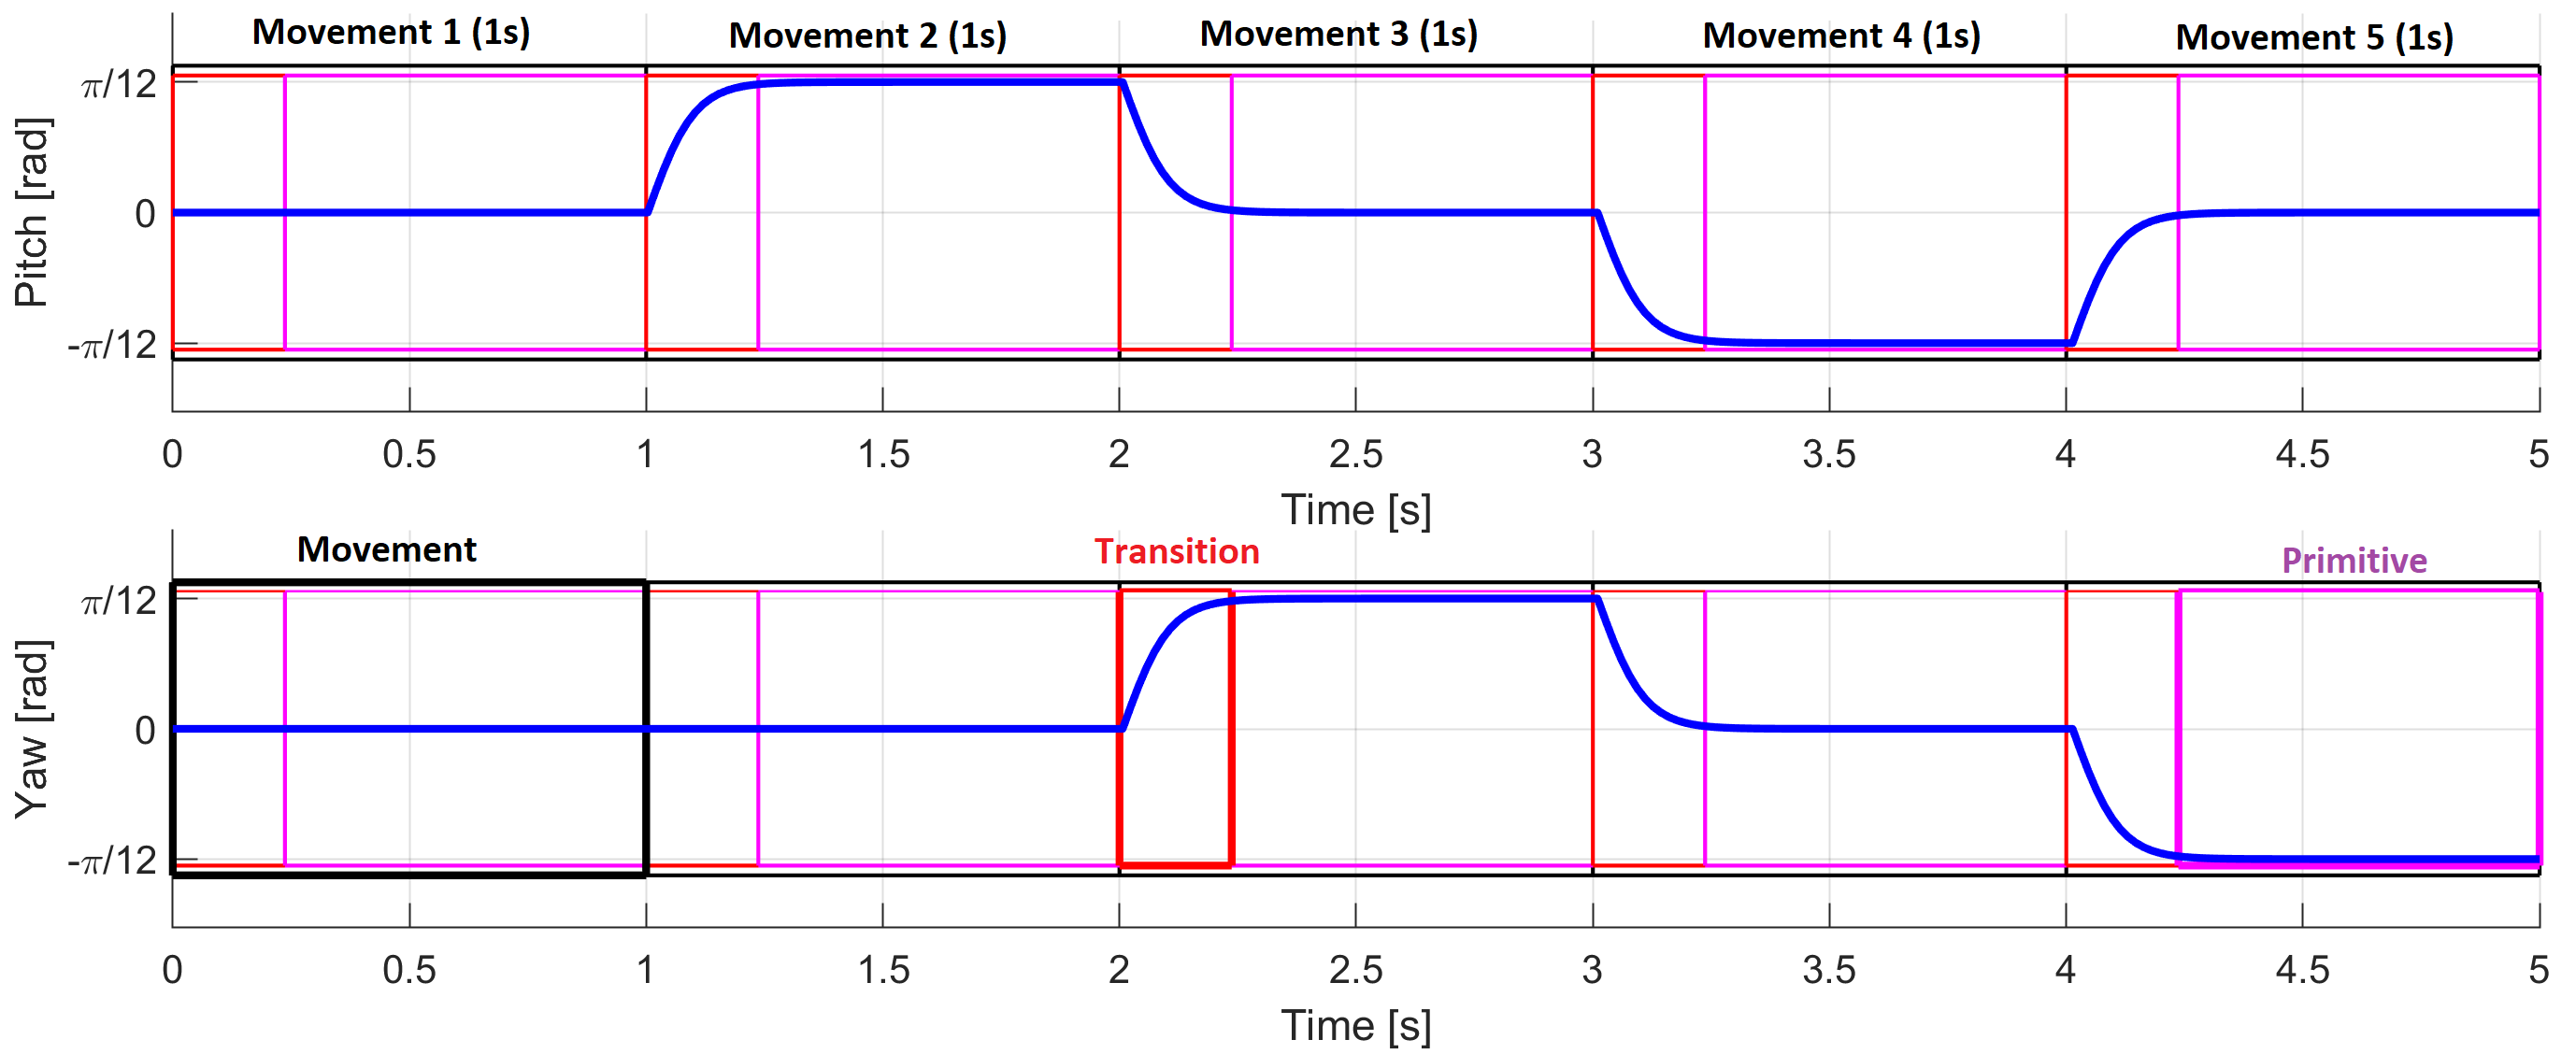
\includegraphics[width=0.95\linewidth]{\FIGDIR/TE062MovementAutomatonExampleWide} 
    \caption{Example of input signal segmentation to movements.}
    \label{fig:movementsExample}
\end{figure}

\begin{note}
    The hybrid automaton (sec. \ref{s:HybridAutomaton}) can be used as the base for simple control mechanism imitating navigators command execution by the pilot. The automaton states can be mapped to primitives and transitions. The reset map needs to be replaced with external order issuer to ensure smooth execution of commands.
    
    The future commands will be stacked in the buffer from which they will be picked for execution.
\end{note}



    \begin{definition}{Movement Primitive:}\label{def:MovementPrimitive}\\\emph{States} from \emph{Hybrid automaton} can be taken as \emph{Movements} in \emph{Movement Automaton}. \emph{MovementPrimitive} (eq. \ref{eq:movementPrimitive}) is describing the \emph{Movement} behavior as transfer function \emph{VectorField} enriched with parameters. 

    \begin{equation}\label{eq:movementPrimitive}
        \begin{aligned}
            &MovementPrimitive(vectorField,minimalDuration,parameters)\\
            &VectorField:SystemState\times parameters \to SystemState
        \end{aligned}
    \end{equation}
    \end{definition}



    \paragraph{Example: }Let say that \emph{UAS} system is given as $\dot{position}=velocity$, then let us have two \emph{MovementPrimitives}:
    
    \begin{enumerate}
        \item \textit{Stay} - $minimalTime=1s$, $parameters=\{\}$, $VectorField:\dot{position}=0$.
        \item \textit{Move} - $minimalTime=1s$, $parameters=\{velocity\}$, $VectorField:\dot{position}=velocity$.
    \end{enumerate}
    
    \paragraph{Trajectory from Movement Primitives:} The \emph{UAS} should \emph{Move} for $5s$ with velocity $10 m/s$, then \emph{Stay} for $10s$, then move for $7s$ with velocity $4 m/s$, with initial position $position_0=0$ and initial time $t_0=1$ The standard approach is to derive transfer function $position = \Theta(\dots)$
    \begin{equation}\label{eq:trajectoryExample}
        position(t)=\Theta(\dots)
        \begin{cases}
            t \in [0,5] &: 10\times t + position(0)\\
            t \in (5,15] &: 0\times (t-5) + position(5)\\
            t \in (15,22]&: 4\times (t-15) + position(15)
        \end{cases}
    \end{equation}

    The \emph{example} given by (eq. \ref{eq:trajectoryExample}) is fairly primitive, but imagine UAS system given by nonlinear dynamics \cite{fossen2011mathematical}. Then defining transfer function for a given command chain can be impossible.

    \begin{definition}{Movement Transition:}\label{def:movementTransition}\\
        \emph{System state} can be different from intended movement application, the notion of \emph{Transition} is therefore introduced as stabilizing element in movement chaining (eq. \ref{eq:movementTransition}).
        \begin{equation}\label{eq:movementTransition}
            Transition:MovementPrimitive\times SystemState \to MovementPrimitive    
        \end{equation}
    \end{definition}

    \paragraph{Trajectory with Transitions:} Introducing two transitions $Transition(Move,Stay)$ and $Transition(Stay,Move)$ reflecting periods when vehicle stop moving or speed-up to desired velocity. The transfer function (eq. \ref{eq:trajectoryExample}) can be rewritten as combination of \emph{MovementPrimitives} (eq. \ref{eq:movementPrimitive}) and \emph{Transitions} (eq. \ref{eq:movementTransition}):
    
    \begin{multline}
        Transition(Stay,Move), Move(5s,10m/s),\\
        Transition(Move,Stay), Stay(10s),\\ 
        Transition(Stay,Move), Move(7s,4m/s)
    \end{multline}.

    \begin{note} There are two types of \emph{movement primitives}:
    \begin{enumerate}
        \item \emph{Stationary} - when the system state is considered neutral, and they are considered an entry point for automaton.
        \item \emph{Dynamic} - when the system state is considered evolving, and they need to be terminated with a \emph{stationary} transition.
    \end{enumerate}
    \end{note}

    \paragraph{Movement Mapping Example:} Transition/MovementPrimitive pairs (eq. \ref{eq:movementTransition}) can be mapped into movements (eq. \ref{eq:movementMappingExample}).
    
    \begin{equation}\label{eq:movementMappingExample}
    \begin{aligned}
        Move(5s,10m/s) &:Transition(Stay,Move), Move(5s,10m/s),\\
        Stay(10s) &: Transition(Move,Stay), Stay(10s),\\ 
        Move(7s,4m/s) &: Transition(Stay,Move), Move(7s,4m/s)
    \end{aligned}    
    \end{equation}

    \begin{definition}{Movement:}\label{def:Movement}\\
        Movement can consist from multiple \emph{Transitions} (eq. \ref{eq:movementTransition}) and one \emph{MovementPrimitive} (eq. \ref{eq:movementPrimitive}), the duration of \emph{MovementPrimitive} can be shortened by \emph{Transitions} duration. \emph{Movement} is defined as follows:
        
        \begin{equation}
            \small Movement \left(
                \begin{gathered}
                    \scriptstyle initialState,\\
                    \scriptstyle initialTime[0..1],\\ 
                    \scriptstyle duration,\\ 
                    \scriptstyle parameters[0..1]
                \end{gathered}\right)
            = \small Chain \left(
            \begin{gathered}
            \small InitialTransition(\dots)[0..*],\\
            \small MovementPrimitive\left(
            \begin{gathered}
                \scriptstyle transitionState,\\
                \scriptstyle remainingDuration,\\
                \scriptstyle parameters
            \end{gathered}\right)\\
            \small LeaveTransition(\dots)[0..*],\\
            \end{gathered}
            \right)
        \end{equation}
        
        \emph{Chain function} connects multiple \emph{initial Transitions} which are applied at \emph{initialState} at \emph{initialTime}. Then own \emph{MovementPrimitive} (eq. \ref{eq:movementPrimitive}) is invoked with \emph{transitionnsState}. \emph{Transitions state} is state changed by \emph{Initial Transitions}. After \emph{Movement Primitive} there can be \emph{Leave Transitions Movement}
    \end{definition}

    \paragraph{Minimal Movement Time:} Given by (eq. \ref{eq:minimalMovementTime}) for \emph{movement} is given as the sum of \emph{MovementPrimitive} (eq. \ref{eq:movementPrimitive}) minimal time, and \emph{Transition} (eq. \ref{eq:movementTransition}) in/out combined minimal time.
    
    \begin{equation}\label{eq:minimalMovementTime}
        minimalTime(Movement)=
        \begin{aligned}
        &minimalTime(MovementPrimitive) +\\ &\text{max}_{in/out}\left\{time(Transition)\right\}
        \end{aligned}
    \end{equation}
   
    \paragraph{Movement Chaining:}\emph{Movements} can be \emph{chained} and applied to initial \emph{system state} to generate \emph{system trajectory}. Example of the trajectory is given by (eq. \ref{eq:trajectoryExample}). Movements are reversibly obtained by participation such a \emph{trajectory} into \emph{Movement primitives} and \emph{Transitions}. Then sample \emph{Trajectory} for $n\in \N^+$ movements looks like (eq. \ref{eq:movementChaining}).
    \begin{equation}\label{eq:movementChaining}
        \begin{aligned}
        &Trajectory(t_0)=State(t_0)\\
        &Trajectory(t_0,t_1]=Movement_1(Trajectory(t_0),t_0,duration_1,parameters_1)\\
        &Trajectory(t_1,t_2]=Movement_2(Trajectory(t_1),t_1,duration_2,parameters_2)\\
        &Trajectory(t_2,t_3]=Movement_3(Trajectory(t_2),t_2,duration_3,parameters_3)\\
        &\vdots\\
        &Trajectory(t_{n-1},t_n]=Movement_n(Trajectory(t_{n-1}),t_{n-1},duration_n,parameters_n)\\
        \end{aligned}
    \end{equation}

    Given \emph{Trajectory} at time $t_0$ is given as the initial \emph{State} of \emph{System}. For time interval $(t_0,t_1)$, which length is equal to $duration_1$, the \emph{State} is given by $Movement_1$ with $parameters_1$ and base time $t_0$. This behavior continues for movements $2,\dots,n$. 

    \begin{definition}{Movement Buffer:}\label{def:MovementBuffer}\\
        \noindent\emph{Movements} can be chained into \emph{Buffer} with the assumption of \emph{continuous movement execution}. \emph{Continuous movement executions} each movement in the chain (eq. \ref{eq:movementChaining}) is executed in time interval $\tau_i=(t_{i-1},t_{i}]$ where $i$ is movement order and $\forall$ $Movement_i$ starting time is $t_0$ or $t_{i-1}$ from the previous movement. With given assumption \emph{Buffer} is given as (eq. \ref{eq:movementBuffer}) with parameters $t_{i-1},t_{i}$ omitted, due $t_0$ and $duration_i$ dependency.
        
        \begin{equation}\label{eq:movementBuffer}
            Buffer = \left\{Movement_i(duration_i,parameters_i)\right\}i\in\N^+
        \end{equation}
    \end{definition}
    
    \begin{definition}{Movement Automaton Trajectory:}\label{def:MovementAutomatonTrajectory}\\
        Let say system \emph{State}$\in\R^n$ which \emph{Trajectory} is defined by movement chaining (eq. \ref{eq:movementChaining}), applied on some \emph{initial time} $t_0\in\R^+$ and final time $t_f=t_0+\sum_{i=1}^{I}duration_i$, with movements contained in \emph{Buffer} (eq. \ref{eq:movementBuffer}) is given as \emph{Trajectory} (eq. \ref{eq:TrajectoryDefinition}).
        
        \begin{equation}\label{eq:TrajectoryDefinition}
            Trajectory(t_0,State(t_0),Buffer)\text{ or } Trajectory(State_0,Buffer) \text{ if } t_0=0
        \end{equation}
    \end{definition}


    \begin{note}
        The space dimension of \emph{Trajectories} is $\R^{n+1}$ if the space dimension of state \emph{Space} is $R^n$, because \emph{Trajectory space} contains evolution of \emph{Space} in time interval $T[t_0,t_f]$.
        
        \noindent The transformation from \emph{transfer function} (eq. \ref{eq:trajectoryExample}) to \emph{trajectory} (eq. \ref{eq:TrajectoryDefinition}) is natural, only set of \emph{Movement primitives} (eq. \ref{eq:movementPrimitive}) and set of \emph{Transitions} (eq. \ref{eq:movementTransition}) is required.
    \end{note}

    \paragraph{State Projection:} \emph{Trajectory} (eq. \ref{eq:TrajectoryDefinition}) is natural evolution of space over time, then there exists \emph{StateProjection} function (eq. \ref{eq:stateprojection}) which returns \emph{State} for specific \emph{Time}.
    
    \begin{equation}\label{eq:stateprojection}
        StateProjection:Trajectory\times Time \to State(Time)
    \end{equation}

